Para controlar el giro de un servo de una placa Arduino, realizaremos las
siguientes conexiones:

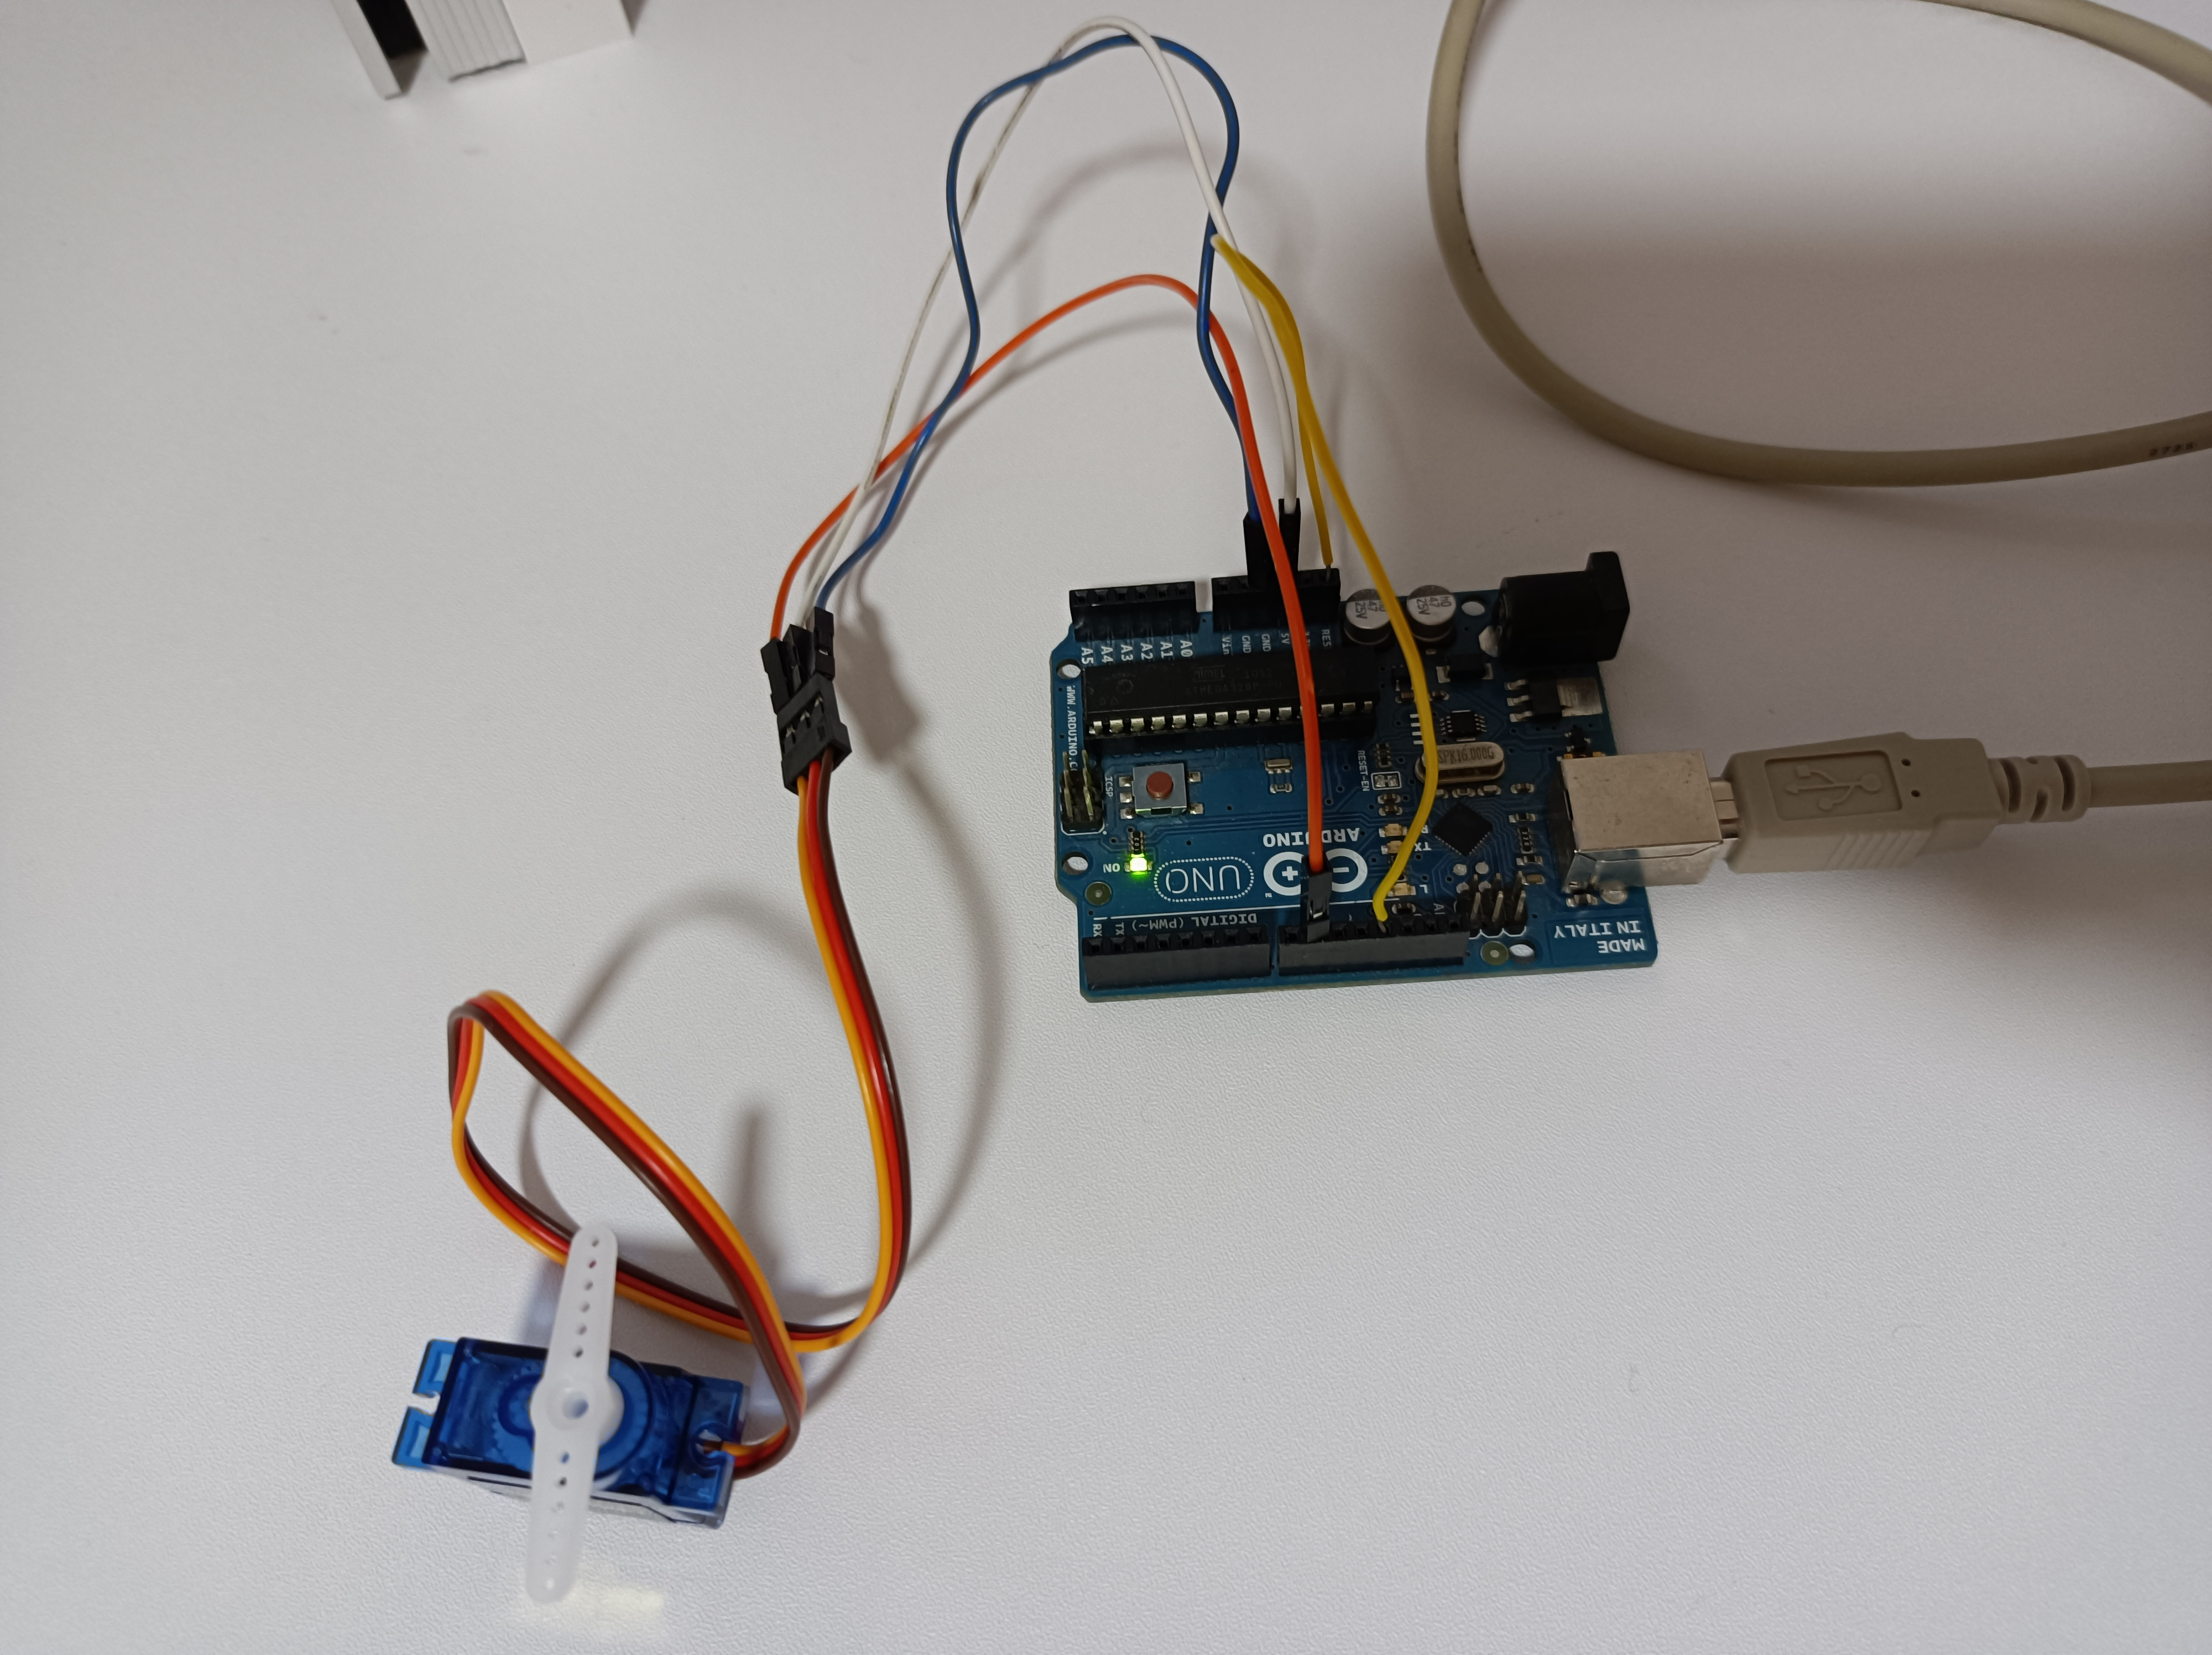
\includegraphics[width=\linewidth]{turn-servo-wiring.jpg}

La placa recibirá el valor en un byte bruto por el puerto serie y lo aplicará
directamente con ayuda de la librería que hace de controlador del motor.

\lstinputlisting[language=C++, caption=turn-servo.ino]{
    1/turn-servo/turn-servo.ino
}

Desde el ordenador se enviará por el puerto serie el valor en bruto,
validando la entrada para que no envíe valores que no estén entre 0 y 180.
Para este ejercicio no necesitamos la librería \verb|console|, por lo que
podemos prescindir de ella. Llamaremos al proyecto del programa cliente
\verb|turn-servo|.

\lstinputlisting[caption=turn-servo/Cargo.toml]{
    1/turn-servo/Cargo.toml
}

\lstinputlisting[language=Rust, caption=turn-servo/src/main.rs]{
    1/turn-servo/src/main.rs
}